\chapter{상태 방정식, 복사와 진공 에너지}

\lectureoverview{균일한 우주의 역사는 대체로 척도인자 \(a(t)\)의 역사다. 프리드만 방정식은 기하를 정하지만, 공간이 팽창할 때 에너지 밀도가 어떻게 변하는지는 물질의 상태 방정식이 알려 준다. 먼저 유체가 한 일을 이용해 \(\rho\propto a^{-3(1+w)}\)를 유도하고, 광자의 운동량 전달을 세어 복사에 대해 \(P=\rho/3\)를 얻은 다음, 마지막으로 \(P=-\rho\)을 통해 진공 에너지를 확인한다. 양의 진공 에너지는 드시터 팽창을 일으킨다. 곡률과 우주상수의 부호에 따라 반동과 재붕괴 해가 생기며, 이를 간단한 역학계로 해석할 수 있다.}

\section{척도인자와 빠져 있는 물질 법칙}

먼저 지금까지의 내용을 되짚어 보자. 균일성과 등방성을 가정하면, 우주의 주요 역사는 하나의 함수 \(a(t)\)에 담긴다. 이 함수를 안다고 해서 우주의 모든 질문에 답할 수 있는 것은 아니지만, 거리와 팽창률, 그리고 대규모 시대의 순서를 결정할 수 있다. 이번 강의의 목적은 아직 관측을 통해 그런 시대를 확립하는 데 있지 않다. 가능한 모형을 만드는 상태 방정식을 기초 물리에서 유도하는 것이 목적이다.

앞서 두 가지 기준 모형을 살펴보았다.
\begin{equation}
a(t)\propto t^{2/3}
\qquad\text{(matter domination)},
\end{equation}
그리고
\begin{equation}
a(t)\propto t^{1/2}
\qquad\text{(radiation domination)}.
\end{equation}
두 법칙 모두 모든 시간에 정확히 성립하지는 않는다. 복사는 초기 시간의 유용한 근사이고, 물질은 그보다 늦은 중간 시기의 근사다. 진공 에너지는 훨씬 뒤에 다시 거동을 바꾼다. 지금 당장 물을 질문은 관측으로 이런 시대를 어떻게 알아내는지가 아니라, 프리드만 방정식의 우변에서 해당 항들을 어떻게 구별하는가이다.

\begin{figure}[htbp]
\centering
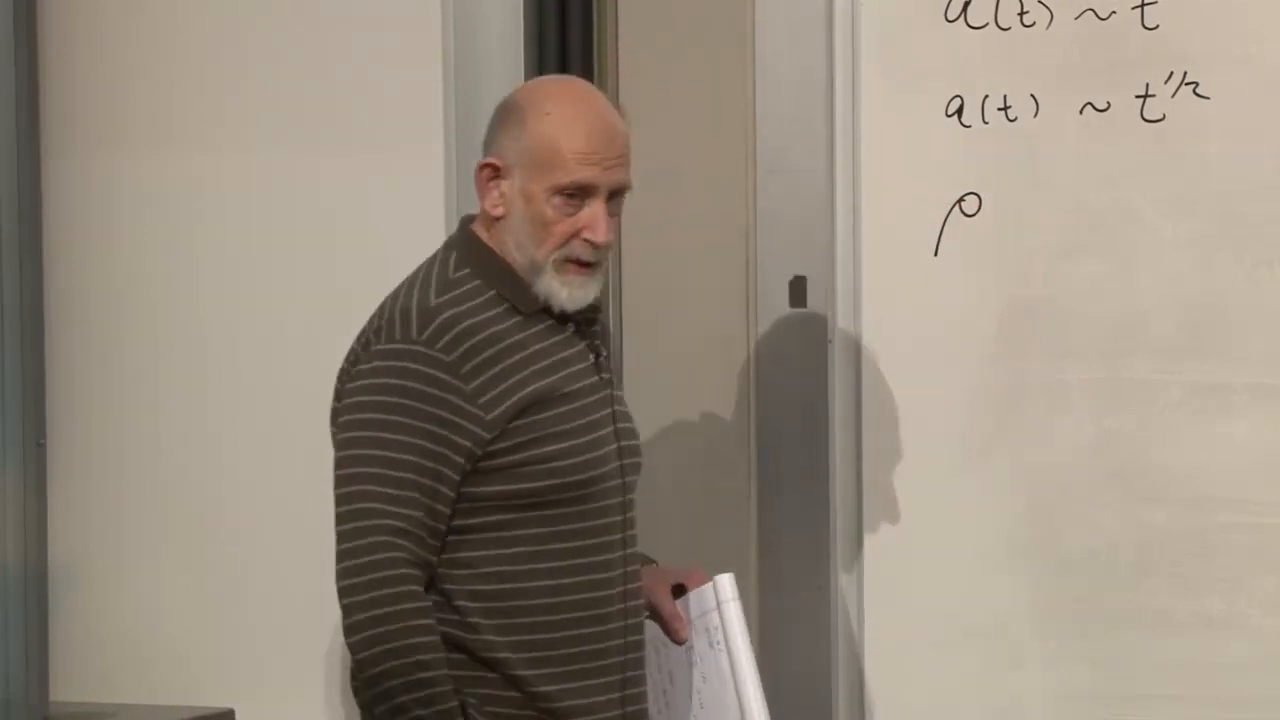
\includegraphics[width=0.72\textwidth]{lecture_05_figure_02.png}
\caption{검토한 척도인자의 거듭제곱 법칙과 새로 도입한 밀도 기호. 완결된 유도가 아니라 다음 내용으로 넘어가는 중간 단계의 판서다.}
\label{fig:c05-review-board}
\lectureframe{00:03:18.380}
\end{figure}

빠진 연결 고리는 상태 방정식이다. 상태 방정식은 프리드만 방정식 우변의 에너지 밀도가 척도인자에 따라 어떻게 변하는지 결정한다. 두 가지 기준 법칙은 다음과 같다.
\begin{equation}
\rho_{\text{matter}}=\frac{\rho_0}{a^3},
\qquad
\rho_{\text{rad}}=\frac{\rho_0}{a^4}.
\label{eq:c05-benchmark-densities}
\end{equation}
물질은 부피에 따라 희석되고, 부피는 \(a^3\)에 비례한다. 복사의 밀도는 여기에 \(a\)만큼의 역수를 더 곱한 것처럼 감소한다. 두 규칙이 압력과 에너지 밀도의 관계에서 어떻게 나오는지 알아보자.

\section{압력에서 밀도 스케일링 법칙으로}

상태 방정식에는 일반적으로 밀도, 압력, 온도와 그 밖의 변수가 들어갈 수 있다. 여기서 다루는 우주론적 성분에는 다음과 같은 유용한 상수-\(w\) 형태를 가정하자.
\begin{equation}
P=w\rho,
\label{eq:c05-eos}
\end{equation}
여기서 \(w\)는 유체의 특성을 나타낸다. 판서에서는 대문자 \(W\)를 쓰지만, 여기서는 관례에 따라 소문자 \(w\)를 쓴다. 이 선형식은 아래의 중요한 사례들을 다루지만, 모든 가능한 유체가 따르는 법칙이 아니라 단순화한 가정이다.

비상대론적 물질에서는 에너지 밀도의 대부분이 정지 에너지다. \(n\)가 수밀도이고 \(m\)이 입자 질량이면, 대략
\begin{equation}
\rho\simeq nmc^2.
\end{equation}
이다. 인자 \(c^2\) 때문에 정지 질량이 작더라도 막대한 에너지 저장고가 된다. 먼지 한 알이 완전히 소멸하면 거시적인 양의 에너지가 방출될 수 있다. 반면 압력은 입자가 벽에 부딪힐 때 운동량을 전달하면서 생기며, 그 크기는 \(nmv^2\) 정도다. 볼링공은 탁구공보다 더 큰 운동량을 전달하지만, 차가운 기체에서는 관련된 모든 속도가 \(v\ll c\)를 만족한다. 따라서
\begin{equation}
\frac{P}{\rho}\sim\frac{v^2}{c^2}\ll1,
\qquad
w\simeq0.
\label{eq:c05-dust-eos}
\end{equation}
이다. 복사는 \(c\)로 움직이므로 이 근사가 적용되지 않는다. 복사의 \(w\)는 가정하지 않고 유도하겠다.

이제 상태 방정식~\eqref{eq:c05-eos}을 \(\rho\)의 스케일링 법칙으로 바꾸는 일반적인 방법이 필요하다. 실험실의 상자 하나면 충분하다. 은하를 실제로 상자에 넣을 수는 없지만, 거친 평균을 취하면 은하는 입자처럼 거동하며 에너지와 압력의 관계를 국소적으로 유도할 수 있다.

\begin{figure}[htbp]
\centering
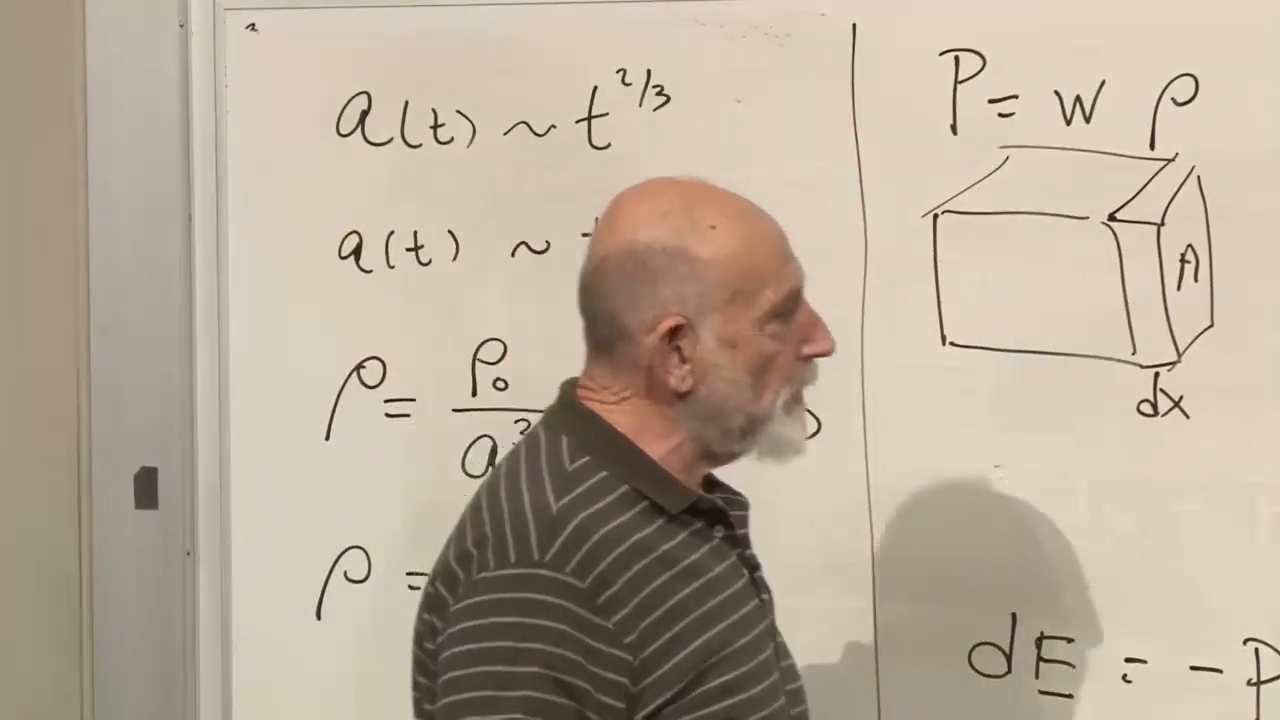
\includegraphics[width=0.86\textwidth]{lecture_05_figure_03.png}
\caption{상태 방정식, 검토한 밀도 스케일링, 열역학적 상자를 한 판서에 담았다. 강사가 앞서 쓴 내용의 일부를 가리므로, 그림은 완전한 필사본이 아니라 배치와 보이는 방정식을 확인하는 용도로 사용한다.}
\label{fig:c05-box-board}
\lectureframe{00:13:39.612}
\end{figure}

판서 왼쪽에는 앞서 살펴본 우주론적 스케일링이 있고, 오른쪽에서는 상자를 이용한 논증이 시작된다. 보이는 내용을 함께 읽으면 다음 관계가 이어진다.
\begin{equation}
\rho_{\text{matter}}=\frac{\rho_0}{a^3},
\qquad
\rho_{\text{rad}}=\frac{\rho_0}{a^4},
\qquad
P=w\rho.
\end{equation}
상태 방정식에서 두 밀도 법칙을 유도하는 것이 우리의 과제다.

한쪽 벽의 면적은 \(A\)이다. 벽을 \(dx\)만큼 바깥으로 옮기면,
\begin{equation}
dV=A\,dx.
\end{equation}
이다. 압력은 단위 면적당 힘이므로 벽에 작용하는 힘은 \(PA\)이다. 기체는 \(PA\,dx=P\,dV\)만큼 일을 하고, 안에 남은 에너지는 감소한다.
\begin{equation}
dE=-P\,dV.
\label{eq:c05-work-law}
\end{equation}
\begin{figure}[htbp]
\centering
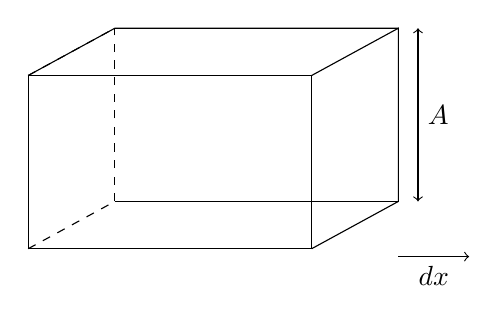
\begin{tikzpicture}[scale=1.0]
\draw (0,0) -- (3.6,0) -- (3.6,2.2) -- (0,2.2) -- cycle;
\draw (3.6,0) -- (4.7,0.6) -- (4.7,2.8) -- (3.6,2.2);
\draw (0,2.2) -- (1.1,2.8) -- (4.7,2.8);
\draw (1.1,0.6) -- (4.7,0.6);
\draw[dashed] (0,0) -- (1.1,0.6);
\draw[dashed] (0,2.2) -- (1.1,2.8);
\draw[dashed] (1.1,0.6) -- (1.1,2.8);
\draw[<->] (4.95,0.6) -- (4.95,2.8);
\node[right] at (4.95,1.7) {\(A\)};
\draw[->] (4.7,-0.1) -- (5.6,-0.1);
\node[below] at (5.15,-0.1) {\(dx\)};
\end{tikzpicture}
\caption{면적이 \(A\)이고 변위가 \(dx\)인 열역학적 상자를 깔끔하게 다시 그린 그림.}
\label{fig:c05-box-redraw}
\end{figure}

전체 에너지는
\begin{equation}
E=\rho V.
\end{equation}
이다. 미분하면
\begin{equation}
d(\rho V)=\rho\,dV+V\,d\rho.
\end{equation}
이다. 이를 방정식~\eqref{eq:c05-work-law}에 대입하면
\begin{equation}
\rho\,dV+V\,d\rho=-P\,dV.
\end{equation}
이다. \(P=w\rho\)를 대입하면
\begin{equation}
V\,d\rho=-(1+w)\rho\,dV.
\end{equation}
을 얻는다. 이 결과는 유용한 방정식에 거의 도달했지만 아직 완성되지는 않았다. \(\rho V\)로 나누자.
\begin{equation}
\frac{d\rho}{\rho}=-(1+w)\frac{dV}{V}.
\end{equation}
\begin{figure}[htbp]
\centering
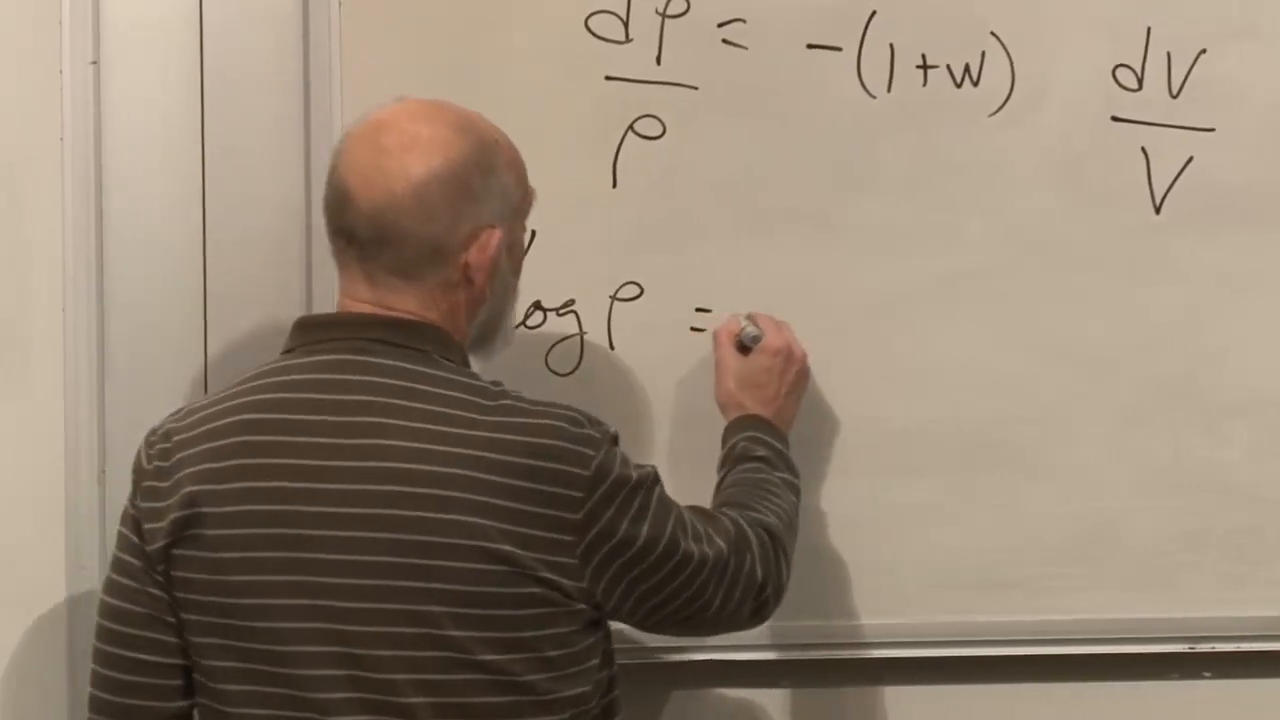
\includegraphics[width=0.78\textwidth]{lecture_05_figure_04.png}
\caption{분리 변수 형태의 밀도-부피 방정식과 로그 적분의 시작 부분. 우변 전체는 앞선 대수 계산을 바탕으로 재구성했으며, 가려진 픽셀에서 읽어 낸 것이 아니다.}
\label{fig:c05-log-board}
\lectureframe{00:15:35.600}
\end{figure}

화면에는 변수분리된 방정식과 \(\log\rho=\)의 시작 부분이 보인다. 적분을 직접 마치면,
\begin{equation}
d(\log\rho)=-(1+w)\,d(\log V),
\end{equation}
따라서
\begin{equation}
\log\rho=-(1+w)\log V+\text{const.}
\end{equation}
이다. 양변에 지수함수를 취하면,
\begin{equation}
\rho\propto V^{-(1+w)}.
\end{equation}
을 얻는다. 이것이 밀도-부피 법칙이다.

이제 상자에서 우주론으로 돌아가자. 벽 하나만 움직인 것은 편리한 유도 방식이었지, 비등방성을 가정한 것이 아니다. 세 방향을 모두 균일하게 팽창시켜도 같은 일의 관계가 나오며, 공변 부피는
\begin{equation}
V\propto a^3.
\end{equation}
에 비례한다. 그러므로
\begin{equation}
\boxed{\rho\propto a^{-3(1+w)}}.
\label{eq:c05-density-scaling}
\end{equation}
이다. \(d\)개의 공간 차원에서는 지수 \(3\)가 \(d\)으로 바뀌며, 나머지 논증은 그대로다.

\section{첫 번째 적용: 물질과 복사}

이제 앞서 살펴본 공식을 가정이 아니라 결과로 다시 얻을 수 있다.

비상대론적 물질에는
\begin{equation}
w=0.
\end{equation}
을 취한다. 그러면
\begin{equation}
\rho\propto a^{-3},
\end{equation}
이며, 이는 물질의 희석 법칙과 정확히 일치한다.

복사에는 일단
\begin{equation}
w=\frac13.
\end{equation}
을 가정하자. 이것이 맞다면,
\begin{equation}
\rho\propto a^{-3(1+1/3)}=a^{-4}.
\end{equation}
이다. 따라서 추가적인 역수 인자는 \(w=1/3\)와 동등하다. 아직 해결되지 않은 단계는 광자의 물리에서 이 값을 유도하는 것이다.

\section{복사 압력이 에너지 밀도의 3분의 1인 이유}

복사는 전자기파로 기술할 수도 있고 질량이 없는 입자로 기술할 수도 있다. 광자를 이용해 상자 안 광자 기체의 압력을 계산하자. 상자는 2차원으로 그려져 있지만, 기체와 그 각도 분포는 3차원이다. 광자는 빛의 속도로 움직이며, 잠정적으로 둔 벽에서 탄성 충돌한다.

우선 모든 광자의 에너지가 같다고 가정하자. 그 값은 \(\epsilon\)이다. 서로 다른 에너지의 기여를 더할 때는 이 단순화가 사라진다. \(\vec{\pi}\)를 광자의 운동량 벡터라 하자. 보통 쓰는 \(p\)는 이미 압력을 나타내는 데 \(P\)를 사용했으므로 쓰지 않는다. 질량이 없는 입자는 다음 관계를 만족한다.
\begin{equation}
\epsilon=c\,\pi,
\end{equation}
여기서 \(\pi=|\vec{\pi}|\)이다. 강의에서 사용하는 단위계에서는 \(c=1\)이므로,
\begin{equation}
\epsilon=\pi.
\end{equation}
이다. \(\nu\)가 광자 수밀도라면 에너지 밀도는
\begin{equation}
\rho=\epsilon\,\nu.
\end{equation}
이다. 한 벽의 법선 방향을 \(x\)축으로 잡자. 그 법선과 각도 \(\theta\)를 이루며 움직이는 광자가 짧은 시간 간격 \(\Delta t\) 동안 벽에 도달하려면, 처음에 두께가 다음과 같은 얇은 층 안에 있어야 한다.
\begin{equation}
\Delta x=\Delta t\cos\theta.
\end{equation}
광자가 반사되면 운동량의 \(x\) 성분은 부호가 뒤집힌다. 따라서 벽에 전달되는 운동량은
\begin{equation}
\Delta \pi_x=2\epsilon\cos\theta.
\end{equation}
이다. 힘은 단위 시간당 운동량 전달량이므로, 충돌 한 번은 \(\Delta \pi_x/\Delta t\)만큼 기여한다. 얇은 층 안의 광자 수는 \(\nu A\Delta x\)이지만, 그중 절반만 벽 쪽으로 움직이므로 관련된 광자 수는 \(\tfrac12 \nu A\Delta x\)이다. 전체 힘을 벽의 면적 \(A\)로 나누면,
\begin{align}
P(\theta)
&=
\frac{1}{A}
\left(\frac{2\epsilon\cos\theta}{\Delta t}\right)
\left(\frac12 \nu A\Delta x\right) \\
&=
\epsilon\nu\cos\theta\frac{\Delta x}{\Delta t} \\
&=
\epsilon\nu\cos^2\theta \\
&=
\rho\cos^2\theta.
\end{align}
을 얻는다. 이 결과는 한 방향으로 움직이는 광자들의 기여만 계산했기 때문에 각도에 따라 달라진다.

\begin{figure}[htbp]
\centering
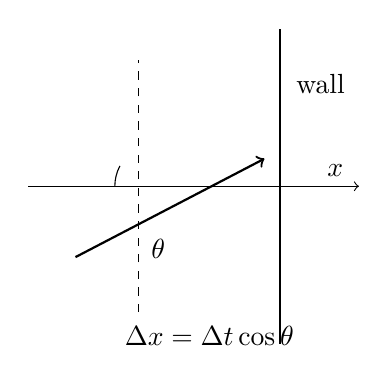
\begin{tikzpicture}[scale=1.0]
\draw[thick] (0,0) -- (0,4);
\draw[->] (-3.2,2) -- (1.0,2);
\node[above] at (0.7,2) {\(x\)};
\draw[dashed] (-1.8,0.4) -- (-1.8,3.6);
\node[below] at (-0.9,0.35) {\(\Delta x=\Delta t\cos\theta\)};
\draw[->,thick] (-2.6,1.1) -- (-0.2,2.35);
\node[below] at (-1.55,1.45) {\(\theta\)};
\draw (-2.1,2) arc[start angle=180,end angle=152,radius=0.55];
\node[right] at (0.08,3.3) {wall};
\end{tikzpicture}
\caption{벽에 각도 \(\theta\)로 입사하는 광자의 운동량과 방사압을 유도하는 데 사용된 기하학적 관계.}
\label{fig:c05-photon-pressure}
\end{figure}

등방 분포에 대해 평균을 취하자. \(\mathbf n=(n_x,n_y,n_z)\)를 광자의 진행 방향을 가리키는 단위벡터라 하자. 그러면
\begin{equation}
n_x=\cos\theta,
\qquad
n_x^2+n_y^2+n_z^2=1.
\end{equation}
이다. 등방 기체에서는 \(n_x^2\), \(n_y^2\), \(n_z^2\)의 평균이 서로 같다. 위 항등식의 평균을 취하면
\begin{equation}
\langle n_x^2\rangle+\langle n_y^2\rangle+\langle n_z^2\rangle=1,
\end{equation}
이며, 대칭성에 따라 각 항이 같으므로
\begin{equation}
\langle n_x^2\rangle=\langle \cos^2\theta\rangle=\frac13.
\end{equation}
이다. 따라서
\begin{equation}
P=\rho\langle \cos^2\theta\rangle=\frac{\rho}{3}.
\end{equation}
이다. 그러므로 복사의 상태 방정식은
\begin{equation}
P=\frac13\rho,
\qquad
w=\frac13.
\end{equation}
이다. 인자 \(1/3\)는 제곱된 단위벡터 성분을 나누어 갖는 공간 방향의 수를 반영한다. 등방적인 \(d\)차원 공간에서는 같은 논증으로 \(\langle n_x^2\rangle=1/d\)를 얻는다. 이로써 서두에서 약속한 미시적 유도가 완성된다.

\subsection{복사 논증을 점검하는 질문}

\begin{classroomqa}
\audiencequestion{모든 광자의 에너지가 같아야 하나요?}
\lecturerresponse{아닙니다. 에너지 구간마다 계산을 따로 하면 됩니다. 각 구간은 그 구간 자체의 에너지 밀도에 대해 3분의 1에 해당하는 압력을 기여하므로, 스펙트럼 전체를 합해도 \(P=\rho/3\)가 유지됩니다. 같은 에너지라고 가정한 것은 표기를 간결하게 하기 위해서였습니다. \lecturetimestamp{00:39:08--00:39:36}}
\end{classroomqa}

\begin{classroomqa}
\audiencequestion{검은 벽이 흡수한다면 완전 거울과 같은 답이 나오나요? 빈 공간에서 벽은 무엇인가요?}
\lecturerresponse{열평형 상태의 검은 벽은 복사를 흡수하고 다시 방출하므로, 평균 운동량 균형은 동일하다. 우주 공간에는 실제 벽이 없으며, 이 표면은 상상으로 설정한 경계다. 바깥쪽으로 나가는 광자마다 등방성에 따라 안쪽으로 들어오는 평균적인 보상 흐름이 있으므로, 국소적인 운동량 흐름 계산은 달라지지 않는다. 교실에서 다룬 복사는 주로 열적 우주 마이크로파 배경 복사이며, 이 경우에는 평형이라는 그림이 특히 자연스럽다. \lecturetimestamp{00:39:37--00:41:19}}
\end{classroomqa}

\begin{classroomqa}
\audiencequestion{양자 통계가 \(P=\rho/3\)를 바꾸나요?}
\lecturerresponse{아닙니다. 보스 통계는 광자가 가능한 모드들을 어떻게 채우는지 결정하므로 스펙트럼과 전체 \(\rho\)를 정하지만, 질량이 없는 입자의 등방 응력은 여전히 그 에너지 밀도의 3분의 1이다. \lecturetimestamp{00:41:51--00:42:02}}
\end{classroomqa}

\begin{classroomqa}
\audiencequestion{광자끼리 산란한다면 어떻게 되나요?}
\lecturerresponse{일반적인 광자-광자 산란은 매우 약하므로 여기서 생기는 보정은 무시할 수 있다. 온도와 밀도가 충분히 높으면 충돌로 전자-양전자 쌍이 만들어져 유효 입자 구성과 상태 방정식이 달라질 수 있다. 이는 실제 효과지만, 이 논증에서 다루는 경우보다 훨씬 더 뜨거운 영역에 해당한다. \lecturetimestamp{00:42:02--00:43:08}}
\end{classroomqa}

\begin{classroomqa}
\audiencequestion{벽의 면적 \(A\)는 어떻게 된 건가요?}
\lecturerresponse{중간 단계의 곱은 광자 하나가 주는 힘과 벽에 부딪히는 광자 수이며, 그 수는 \(A\)에 비례한다. 압력은 힘을 면적으로 나눈 값이므로 마지막에 나누는 과정에서 \(A\)가 약분된다. 중간 식을 너무 일찍 압력이라고 부른 것이 판서에서 빠진 부분이었다. 힘을 압력으로 바꾸는 단계를 복원하면 문제가 해결된다. \lecturetimestamp{00:43:11--00:44:01}}
\end{classroomqa}

\section{음압과 장력의 의미}

지금까지는 입자가 벽에 부딪혀 벽을 바깥쪽으로 밀었다. 이 그림은 자연스럽게 양압을 낳지만, 가능한 경우를 모두 아우르지는 않는다.

\begin{classroomqa}
\audiencequestion{에너지 밀도 자체가 음수일 수 있나요?}
\lecturerresponse{양자론에서는 제한된 상황에서 음의 에너지 밀도가 허용되며, 우주상수도 형식적으로는 어느 부호든 가질 수 있다. 이런 경우에는 신중한 취급이 필요하므로, 여기서 바로 출발하지는 않겠다. 더 익숙한 출발점은 음의 \emph{압력}이며, 에너지 밀도가 양수인 동안에도 생길 수 있다. \lecturetimestamp{00:44:25--00:44:59}}
\end{classroomqa}

\begin{classroomqa}
\audiencequestion{압력이 어떻게 음수가 될 수 있나요?}
\lecturerresponse{1차원 세계에서 상자는 선분이다. 자유롭게 움직이는 입자들은 양 끝에서 튕겨 나와 바깥쪽으로 밀므로 양압이 생긴다. 대신 양 끝을 팽팽한 끈이나 용수철로 연결해 보자. 양 끝을 바깥쪽으로 당기면 용수철은 안쪽으로 당긴다. 이 안쪽 방향의 힘이 장력이며, 음압을 나타내는 1차원 모형이다. \lecturetimestamp{00:45:04--00:46:31}}
\end{classroomqa}

\begin{figure}[htbp]
\centering
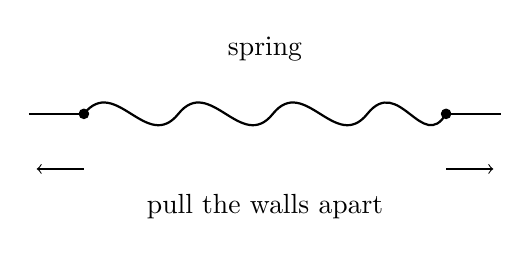
\begin{tikzpicture}[scale=1.0]
\draw[thick] (-3,0) -- (-2.3,0);
\draw[thick] (2.3,0) -- (3,0);
\draw[fill] (-2.3,0) circle (0.06);
\draw[fill] (2.3,0) circle (0.06);
\draw[thick] (-2.3,0)
.. controls (-1.9,0.5) and (-1.5,-0.5) .. (-1.1,0)
.. controls (-0.7,0.5) and (-0.3,-0.5) .. (0.1,0)
.. controls (0.5,0.5) and (0.9,-0.5) .. (1.3,0)
.. controls (1.7,0.5) and (2.0,-0.5) .. (2.3,0);
\draw[->] (-2.3,-0.7) -- (-2.9,-0.7);
\draw[->] (2.3,-0.7) -- (2.9,-0.7);
\node[below] at (0,-0.9) {pull the walls apart};
\node[above] at (0,0.55) {spring};
\end{tikzpicture}
음압을 비유하는 1차원 용수철.\caption{
}
\label{fig:c05-tension}
\end{figure}

이에 따라 일의 계산도 반대로 된다. 팽창하면 양압을 가진 기체가 일을 하고 내부 에너지를 잃는다. 장력에 맞서 바깥쪽으로 당기면 용수철에 에너지가 저장된다. 더 일반적으로는 서로 끌어당기는 구성 요소가 서로와 경계를 안쪽으로 당길 수 있다. 따라서 모순 없이 \(\rho>0\)이면서 \(P<0\)인 계가 존재할 수 있고, 이때 \(w<0\)이다. 진공 에너지가 바로 이런 부호 조합을 갖기 때문에 이 가능성이 중요하다.

\section{진공 에너지와 우주상수}

진공 에너지는 빈 공간 자체에 속하는 것으로 본다. 양자장론은 장 모드에 대응하는 조화 진동자의 영점 운동을 통해 진공 에너지에 대한 동기를 제공하지만, 거시적인 기술에 그 미시적 문제를 풀 필요는 없다. 정의상 빈 공간의 에너지 밀도는 어느 곳에서 얼마나 큰 영역을 택하든 같다.
\begin{equation}
\rho=\rho_0=\text{const.}
\label{eq:c05-vacuum-density}
\end{equation}
부피가 \(V\)인 영역에 진공 에너지만 들어 있다면, 그 영역의 전체 에너지는
\begin{equation}
E=\rho_0 V.
\end{equation}
이다.
\begin{classroomqa}
\audiencequestion{상자는 허용된 장 모드를 제한해 진공 밀도를 바꾸나요?}
\lecturerresponse{유한한 영역의 부피가 우주 전체보다 작으므로 그 안의 전체 에너지도 우주 전체의 에너지보다 작다. 하지만 부피 밀도 \(\rho_0\)는 그대로다. 실제 경계는 모드 에너지를 바꾸어 카시미르 효과를 일으킬 수 있지만, 그 보정은 간격이 관련 파장과 비슷할 때 중요하다. 이는 우주론에서 다루는 대규모 진공 밀도가 아니다. \lecturetimestamp{00:50:06--00:51:25}}
\end{classroomqa}

다음을 도입하자.
\begin{equation}
\Lambda=\frac{8\pi G}{3}\rho_0.
\label{eq:c05-lambda-definition}
\end{equation}
이 정의는 프리드만 방정식에 나타나는 조합을 하나로 묶는다. 역관계는
\begin{equation}
\rho_0=\frac{3\Lambda}{8\pi G}.
\end{equation}
이다. 매개변수 \(\Lambda\)가 우주상수다. 후기 가속 팽창을 일으키는 거의 일정한 양의 성분은 흔히 암흑 에너지라고 부른다.

척도인자의 의존성은 이미 정해졌으므로, 상자를 이용한 논증을 거꾸로 적용해 압력을 알아내자. \(d\rho_0=0\)이므로,
\begin{equation}
dE=d(\rho_0V)=\rho_0\,dV.
\end{equation}
이다. 한편 열역학적 일의 관계는 여전히
\begin{equation}
dE=-P\,dV.
\end{equation}
이다. \(P=w\rho_0\)라고 쓰면,
\begin{equation}
dE=-w\rho_0\,dV.
\end{equation}
이다. 두 식을 비교하면
\begin{equation}
w=-1.
\end{equation}
을 얻고, 따라서
\begin{equation}
P=-\rho.
\end{equation}
이다. 용수철 비유는 이 부호를 미리 보여 주었다. 양의 진공 에너지는 음압을, 음의 진공 에너지는 양압을 가진다. \(w\)의 천문학적 측정은 후기 우주 성분이 실제로 희석되지 않는 진공처럼 거동하는지를 묻는다. \(w\)가 \(-1\)에 가까울수록 그 거동은 방정식~\eqref{eq:c05-vacuum-density}에 가까워진다.

\begin{classroomqa}
\audiencequestion{\(P=-\rho\)은 빈 우주의 상태 방정식인가요? 그리고 \(\rho_0\)는 계산할 수 있나요?}
\lecturerresponse{진공 에너지가 있을 때 이것은 빈 공간의 상태 방정식이다. 그 크기를 알아내기는 훨씬 어렵다. 아직 발견되지 않은 장을 포함해 모든 양자장과 모든 에너지 척도가 기여할 수 있으므로, 관측값을 설명하는 합의된 계산은 없다. 핵심 수수께끼는 \(w=-1\)라고 쓰는 법이 아니라, 순수한 \(\rho_0\)가 왜 그토록 놀라울 만큼 작은가이다. \lecturetimestamp{00:57:27--00:58:29}}
\end{classroomqa}

\section{프리드만 동역학에서의 진공 에너지}

앞서 순수한 물질과 순수한 복사를 따로 살펴본 것처럼 진공 에너지만 분리해 보자. \(\rho=\rho_0\)이면 프리드만 방정식은 다음과 같이 된다.
\begin{equation}
\left(\frac{\dot a}{a}\right)^2=\Lambda-\frac{k}{a^2},
\label{eq:c05-vacuum-friedmann}
\end{equation}
구면, 평탄, 쌍곡 공간에서 \(k=+1,0,-1\)이다. \(\Lambda\)의 두 가지 부호와 \(k\)의 세 가지 선택을 조합하면 여섯 가지 부호 경우가 나오지만, 모든 경우에 실수해가 존재하는 것은 아니다.

\begin{remark}
강의에서는 \(\Lambda=(8\pi G/3)\rho_0\)로 정의하므로, 여기서 \(\Lambda\)의 차원은 \(H^2\)이다. 흔히 쓰는 규약 \(G_{\mu\nu}+\Lambda_{\mathrm E}g_{\mu\nu}=8\pi G T_{\mu\nu}\)에서는 이에 대응하는 매개변수가 \(\Lambda_{\mathrm E}=3\Lambda\)이다.
\end{remark}

\subsection{평탄한 드시터 팽창}

\(k=0\)로 놓으면,
\begin{equation}
\left(\frac{\dot a}{a}\right)^2=\Lambda.
\end{equation}
이다. \(\Lambda>0\)일 때 팽창하는 가지를 택하면,
\begin{equation}
\dot a=\sqrt{\Lambda}\,a,
\end{equation}
이고, 따라서
\begin{equation}
a(t)=C\,e^{\sqrt{\Lambda}\,t}.
\end{equation}
이다. 그러면 허블 매개변수는 일정하다.
\begin{equation}
H=\frac{\dot a}{a}=\sqrt{\Lambda}.
\end{equation}
이것은 평탄 절단의 드시터 공간이다. 우주상수 해를 찾은 Willem de Sitter의 이름을 딴 것으로, 그가 이 해를 찾은 것은 아인슈타인이 그 항을 도입한 1917 직후였다. \(\Lambda<0\)이고 \(k=0\)이면 방정식~\eqref{eq:c05-vacuum-friedmann}은 실수해가 없다. \(H^2\)는 음수가 될 수 없기 때문이다.

\begin{classroomqa}
\audiencequestion{여기서 허블 매개변수는 정말 일정한가요? 이 시공간에는 빅뱅이 있나요?}
\lecturerresponse{평탄 절단의 순수한 해에서는 \(H=\sqrt{\Lambda}\)가 정확히 일정하다. \(a(t)\to0\)이 \(t\to-\infty\)일 때에만 성립하지만, 이 좌표 패치는 측지선 완비가 아니다. 과거 방향의 일부 궤적은 유한한 고유 시간 안에 경계에 도달한다. 따라서 이 식만으로 전역적인 빅뱅의 존재 여부가 결정되지는 않는다. 완전한 드시터 기하에는 이 평탄 패치보다 더 넓은 영역이 포함되며, 이 문제는 기하를 자세히 살펴볼 때 다루겠다. \lecturetimestamp{01:06:54--01:08:07}}
\end{classroomqa}

물질, 복사, 곡률, 진공 에너지를 포함하는 우주의 프리드만 방정식을 개략적으로 쓰면
\begin{equation}
\left(\frac{\dot a}{a}\right)^2
=
\Lambda+\frac{C_m}{a^3}+\frac{C_r}{a^4}-\frac{k}{a^2}.
\label{eq:c05-mixed-friedmann}
\end{equation}
이다. 초기에는 \(a\)가 작아 역수 거듭제곱 항들이 지배하고 진공 에너지는 무시할 수 있다. 후기에는 \(a\)가 커져 상수항 \(\Lambda\)가 지배한다. 따라서 우주는 전이를 겪는다. 초기에는 물질 또는 복사가 지배하는 것처럼 보이고, 후기에는 드시터와 비슷한 거동에 가까워진다.

지수함수는 \(\ddot a>0\)이므로, 진공 에너지 지배는 가속 팽창이다. 물질이 여전히 방정식~\eqref{eq:c05-mixed-friedmann}에 기여하므로 전이 중의 가속이 정확히 지수적일 필요는 없다. 강의 당시의 관측에 따르면 우주는 이미 순수한 드시터 단계에 들어선 상태가 아니라 이런 경쟁이 진행되는 시기에 관측되고 있다.

\section{진공 에너지에 관한 질문}

\begin{classroomqa}
\audiencequestion{진공 에너지가 바닥 상태 에너지라면 어떻게 음수가 될 수 있나요?}
\lecturerresponse{보손 진동자 모드는 \(+\tfrac12\hbar\omega\)만큼 기여하는 반면, 페르미온 모드는 반대 부호로 기여한다. 진공 에너지는 여러 장과 에너지 척도의 기여를 합한 것이므로, 전체를 알기 전에는 어느 쪽 부호든 가능하다. 기여가 존재한다는 사실은 자연스럽지만, 그 합이 놀라울 정도로 작게 남는 이유를 설명하기는 어렵다. \lecturetimestamp{01:12:00--01:14:12}}
\end{classroomqa}

\begin{classroomqa}
\audiencequestion{일정한 \(w=-1\)이면 미래에 빅립이 생기나요?}
\lecturerresponse{아니다. \(w=-1\)인 우주상수는 드시터와 같은 지수 팽창을 일으키지만, 빅립이라고 부르는 유한 시간의 발산은 일으키지 않는다. 그런 시나리오는 우주가 팽창할수록 밀도가 증가하는 \(w<-1\)의 가상적인 팬텀 성분에 해당한다. 여기서는 그런 성분을 가정하지 않는다. \lecturetimestamp{01:14:13--01:15:50}}
\end{classroomqa}

\begin{classroomqa}
\audiencequestion{정확한 초대칭성이 진공 에너지를 0으로 만들 수 있나요?}
\lecturerresponse{모든 보손 자유도가 페르미온 자유도와 짝을 이루므로 영점 기여를 상쇄할 수 있다. 하지만 자연에는 저에너지에서 정확한 초대칭성이 나타나지 않는다. 관측된 보손과 페르미온은 질량이 같은 짝입자가 아니다. 따라서 정확한 상쇄로는 현재 관측되는 우주의 진공 에너지를 설명할 수 없다. \lecturetimestamp{01:15:51--01:16:20}}
\end{classroomqa}

\begin{classroomqa}
\audiencequestion{자연적인 진공 에너지 추정치와 관측값 사이의 엄청난 차이는 무엇인가?}
\lecturerresponse{보편 상수 \(c\), \(\hbar\), \(G\)는 플랑크 단위를 정한다. 빛의 속도 \(c\)는 모든 신호의 속도를 제한하고, \(\hbar\)는 보편적인 양자 불확정성의 척도를 정하며, \(G\)은 모든 에너지를 중력과 결합시킨다. 이 상수들로 대략 \(10^{-5}\)그램인 플랑크 질량과 대략 \(10^{-33}\)센티미터인 플랑크 길이를 정의할 수 있으며, 이를 바탕으로 플랑크 길이의 세제곱당 플랑크 에너지에 해당하는 대략적인 플랑크 에너지 밀도를 얻는다. 이 단위계에서 관측된 진공 밀도는 강의에서 약 \(10^{-123}\)로 제시되며, 정확한 지수는 관례에 따라 달라진다. 자연스럽게 훨씬 더 큰 규모를 시사하는 기여들이 왜 합쳐져 이처럼 극히 작지만 영이 아닌 결과를 남기는지가 수수께끼다. \lecturetimestamp{01:16:21--01:23:12}}
\end{classroomqa}

\begin{classroomqa}
\audiencequestion{진공 기여가 예상되는데도 물리학자들은 왜 영이 아닌 우주 상수를 발견하고 놀랐는가?}
\lecturerresponse{관측이 거듭 개선되는 동안에도 결과는 계속 영과 양립하는 것으로 나타났다. 이러한 이력은 미래의 양자중력 이론에서 발견될지도 모르는 미지의 정확한 원리가 완전한 상쇄를 강제하리라는 심리적 기대를 키웠다. 결국 검출은 그 기대를 뒤집었다. 놀라움은 점점 더 엄격해진 영 결과가 수십 년간 이어진 데서 비롯된 것이지, 진공 에너지가 반드시 사라져야 한다는 유도 결과에서 비롯된 것이 아니었다. \lecturetimestamp{01:23:14--01:26:05}}
\end{classroomqa}

\begin{classroomqa}
\audiencequestion{관측으로 암흑 에너지가 시간에 따라 변하는지 알아낼 수 있나요?}
\lecturerresponse{먼 미래에 급격한 변화가 일어날 가능성을 배제할 수는 없지만, 수십억 년에 걸친 최근의 팽창 역사는 비교할 수 있다. \(w\), 또는 더 일반적으로 \(w(a)\)를 측정하면 그 기간 동안 밀도가 변했는지 검증할 수 있다. 강의에서는 당시의 제약을 대략 10퍼센트 수준이라고 보고한다. 이 수치는 역사적인 값이며, 계속 유효한 핵심은 \(w=-1\)일 때 밀도가 변하지 않는다는 점이다. \lecturetimestamp{01:26:06--01:27:16}}
\end{classroomqa}

\begin{classroomqa}
\audiencequestion{공간 차원의 수가 달라도 결과가 달라지나요?}
\lecturerresponse{전체적인 구조는 유지된다. 등방적인 \(d\)차원 공간에서 복사는 \(w=1/d\)이고 \(a^{-(d+1)}\)에 따라 희석되는 반면, 로런츠 불변인 진공 에너지는 여전히 \(w=-1\)이다. 프리드만 방정식의 수치 계수는 차원에 따라 달라지지만, 희석되는 물질과 복사, 희석되지 않는 진공의 구분은 그대로 남는다. \lecturetimestamp{01:27:16--01:27:57}}
\end{classroomqa}

\section{곡률과 역학적 비유}

\subsection{양의 진공 에너지에서의 양의 곡률}

\(k=+1\)와 \(\Lambda>0\)을 택하자.
\begin{equation}
\left(\frac{\dot a}{a}\right)^2=\Lambda-\frac{1}{a^2}.
\label{eq:c05-closed-vacuum}
\end{equation}
양변에 \(a^2\)를 곱하면,
\begin{equation}
\dot a^2-\Lambda a^2=-1.
\label{eq:c05-inverted-oscillator}
\end{equation}
이다. \(a\)를 가상의 입자의 좌표로 보자. 그러면 \(\dot a^2\)은 운동에너지 항이고, \(-\Lambda a^2\)는 위로 열린 포물선 형태의 퍼텐셜이며, 전체 에너지는 \(-1\)이다. 물리적으로 허용되는 가지는 \(a\geq\Lambda^{-1/2}\)이다. 우주는 큰 크기에서 수축해 최소점에서 정지한 뒤 다시 팽창한다.

정확한 해는
\begin{equation}
a(t)=\Lambda^{-1/2}\cosh(\sqrt{\Lambda}\,t).
\label{eq:c05-closed-desitter}
\end{equation}
이다. 다음 식을 이용하면
\begin{equation}
\cosh(\sqrt{\Lambda}\,t)
=
\frac12\left(e^{\sqrt{\Lambda}\,t}+e^{-\sqrt{\Lambda}\,t}\right),
\end{equation}
이 함수는 시간에 대해 대칭이다. \(t=0\)일 때 \(a=\Lambda^{-1/2}\)이며, 시간의 양방향으로 멀어질수록 지수적으로 커진다. 따라서 닫힌 절단에서는 수축, 특이점이 없는 최소 크기, 재팽창이 나타난다. 이는 평탄한 지수 절단과 전역적으로는 달라 보이지만, 두 좌표계 모두 같은 드시터 기하의 일부를 덮는다.

\subsection{음의 우주상수}

\(\Lambda=-|\Lambda|\)라고 쓰자. \(k=+1\)이면 방정식~\eqref{eq:c05-vacuum-friedmann}의 우변은 모든 \(a\)에서 음수인 반면, \(H^2\geq0\)이다. 이 순수 진공 유형에는 실수 FRW 해가 존재하지 않는다.

\(k=-1\)이면,
\begin{equation}
\left(\frac{\dot a}{a}\right)^2=-|\Lambda|+\frac{1}{a^2}.
\end{equation}
이다. 양변에 \(a^2\)를 곱하면,
\begin{equation}
\dot a^2+|\Lambda|a^2=1.
\label{eq:c05-negative-lambda-oscillator}
\end{equation}
이다. 이것은 조화 진동자의 에너지 방정식이다. \(a\geq0\)이므로 물리적인 반주기는
\begin{equation}
a(t)=\frac{1}{\sqrt{|\Lambda|}}
\sin\!\left(\sqrt{|\Lambda|}\,t\right),
\qquad
0<t<\frac{\pi}{\sqrt{|\Lambda|}}.
\end{equation}
이다. 열린 우주는 \(a=0\)에서 시작해 \(a_{\max}=|\Lambda|^{-1/2}\)에 도달한 뒤 빅 크런치로 돌아간다. 따라서 열린 공간의 기하가 영원한 팽창을 보장하지는 않는다. 음의 우주상수는 팽창을 되돌릴 수 있다. 매우 큰 양의 \(\Lambda\)는 중력적으로 묶인 구조를 찢어 놓고, 큰 음의 값은 빠른 재붕괴를 일으킨다.

\begin{figure}[htbp]
\centering
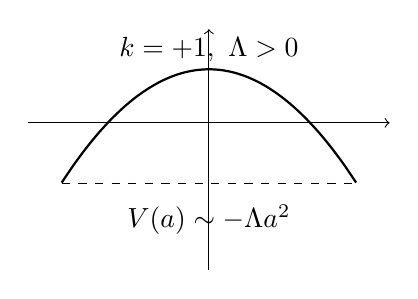
\begin{tikzpicture}[scale=0.85]
\draw[->] (-2.7,0) -- (2.7,0);
\draw[->] (0,-2.2) -- (0,1.4);
\draw[thick,domain=-2.2:2.2,smooth] plot (\x,{-0.35*(\x)^2 + 0.8});
\draw[dashed] (-2.2,-0.9) -- (2.2,-0.9);
\node at (0,-1.45) {\(V(a)\sim -\Lambda a^2\)};
\node at (0,1.1) {\(k=+1,\ \Lambda>0\)};
\end{tikzpicture}
\hspace{2em}
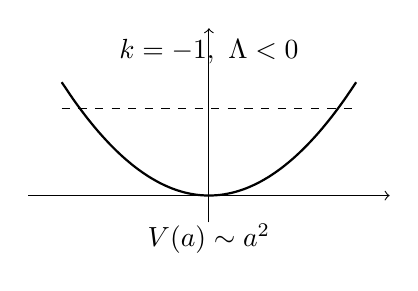
\begin{tikzpicture}[scale=0.85]
\draw[->] (-2.7,0) -- (2.7,0);
\draw[->] (0,-0.4) -- (0,2.5);
\draw[thick,domain=-2.2:2.2,smooth] plot (\x,{0.35*(\x)^2});
\draw[dashed] (-2.2,1.3) -- (2.2,1.3);
\node at (0,-0.65) {\(V(a)\sim a^2\)};
\node at (0,2.15) {\(k=-1,\ \Lambda<0\)};
\end{tikzpicture}
\caption{닫힌 드 시터 바운스와 열린 우주에서 음의 \(\Lambda\)로 일어나는 재붕괴를 나타낸 개략적 유효 퍼텐셜.}
\label{fig:c05-mechanical-potentials}
\end{figure}

\begin{classroomqa}
\audiencequestion{이 프리드만 방정식은 정말 아인슈타인 방정식인가요?}
\lecturerresponse{그렇습니다. 균질성과 등방성으로 계량이 단일 함수 \(a(t)\)로 줄어든 뒤의 아인슈타인 장방정식입니다. 대칭성에 따른 축약으로 텐서 성분 대부분이 사라지고, 우주 팽창을 나타내는 이 상미분방정식이 남습니다. \lecturetimestamp{01:43:52--01:44:05}}
\end{classroomqa}

\begin{classroomqa}
\audiencequestion{스케일 인자 \(a\)는 복소수일 수 있나요?}
\lecturerresponse{여기서 다루는 실수 고전 FRW 우주론에서는 그렇지 않습니다. 스케일 인자는 공간의 크기를 나타내므로 실수이며 음이 아닌 값으로 둡니다. 다른 수학적 접근에서는 복소화된 기하가 등장할 수 있지만, 이 강의의 해에서는 다루지 않습니다. \lecturetimestamp{01:44:06--01:44:21}}
\end{classroomqa}

\begin{classroomqa}
\audiencequestion{압력이 밀도의 선형 함수여야 하는 물리적 이유가 있나요?}
\lecturerresponse{아닙니다. \(w\)가 일정하면 다루기 편하고, 여기서 고려하는 주요 성분들을 실제로 기술할 수 있습니다. 물질, 복사, 진공의 혼합물은 모든 시대에 걸쳐 하나의 일정한 \(w\)를 갖지 않으며, 일반적인 물질은 비선형적인 \(P(\rho)\) 관계를 가질 수 있습니다. 압력이 밀도만의 함수인 유체에서는 \(dP/d\rho\)가 음속의 제곱을 결정하며, 단위계에서 \(c=1\)로 두면 일정한 \(w\)에 따라 그 도함수도 일정해지지만, 자연이 반드시 그래야 하는 것은 아닙니다. \lecturetimestamp{01:44:21--01:45:34}}
\end{classroomqa}

\section{기억해 둘 내용}

상태방정식은 미시적 물리와 스케일 인자의 시간에 따른 이력을 연결합니다. 공변 상자에서 단열적으로 일을 하면
\[
\rho\propto a^{-3(1+w)}.
\]
차가운 물질은 \(w=0\)이고 \(\rho\propto a^{-3}\)입니다. 광자 운동량의 등방적 흐름은 다음을 줍니다.
\[
\left\langle\cos^2\theta\right\rangle=\frac13,
\qquad
P_{\mathrm r}=\frac{\rho_{\mathrm r}}{3},
\qquad
\rho_{\mathrm r}\propto a^{-4}.
\]

장력은 음압을 물리적으로 이해할 수 있게 해 줍니다. 일정한 진공 밀도는 다음을 만족합니다.
\[
P_\Lambda=-\rho_\Lambda,
\qquad
w_\Lambda=-1.
\]
양의 진공 에너지는 평탄한 슬라이싱에서 지수적인 드시터 팽창을 일으키며, 닫힌 슬라이싱에서는 \(\cosh\) 바운스를 일으킵니다. 음의 진공 에너지는 열린 우주조차 다시 붕괴하게 만들 수 있습니다. 부호가 어느 경우든 프리드만 방정식은 유효한 역학적 에너지 방정식으로 읽을 수 있습니다. 아직 풀리지 않은 질문은 양자장이 왜 진공 에너지에 기여하는가가 아니라, 관측된 순기여가 정확히 0은 아니면서도 왜 거의 0인가입니다.
